% !TeX program = pdflatex
\documentclass[tikz,border=8pt]{standalone}
\usepackage{tikz}
\usetikzlibrary{positioning}
\definecolor{FigureBlue}{HTML}{2563EB}
\definecolor{FigureOrange}{HTML}{EA580C}
\definecolor{FigureGreen}{HTML}{16A34A}
\definecolor{FigureSlate}{HTML}{64748B}
\begin{document}
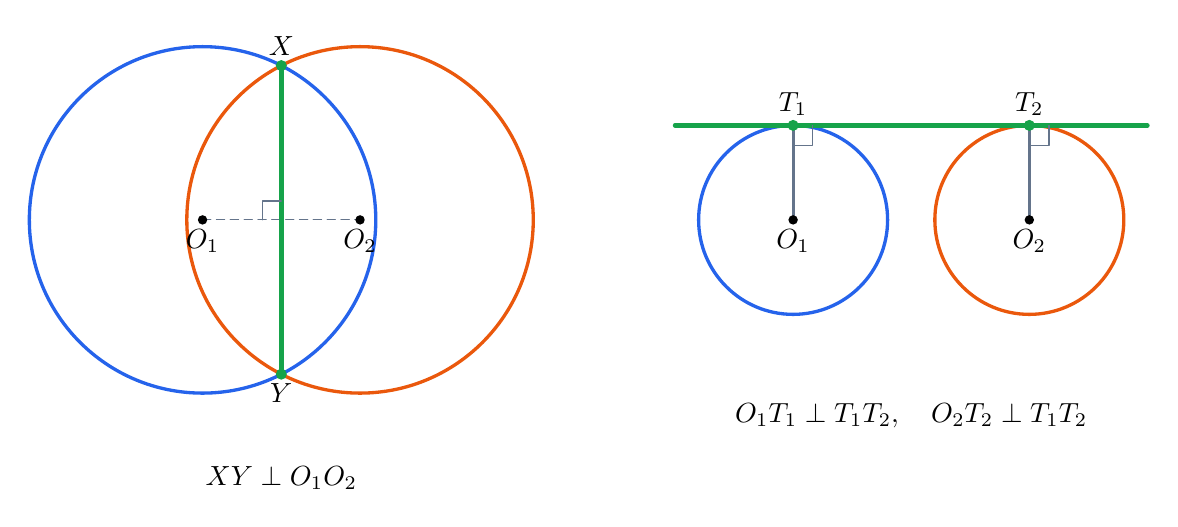
\begin{tikzpicture}[line cap=round,line join=round]
  \begin{scope}
    \coordinate (O1) at (-1,0);\coordinate (O2) at (1,0);
    \coordinate (X) at (0,1.959592);\coordinate (Y) at (0,-1.959592);
    \draw[FigureBlue,line width=1.2pt] (O1) circle[radius=2.2];
    \draw[FigureOrange,line width=1.2pt] (O2) circle[radius=2.2];
    \draw[FigureSlate,densely dashed] (O1)--(O2);
    \draw[FigureGreen,line width=1.6pt] (X)--(Y);
    \fill (O1) circle (1.7pt);\fill (O2) circle (1.7pt);\fill[FigureGreen] (X) circle (2pt);\fill[FigureGreen] (Y) circle (2pt);
    \node[below] at (O1) {$O_1$};\node[below] at (O2) {$O_2$};\node[above] at (X) {$X$};\node[below] at (Y) {$Y$};
    \draw[FigureSlate] (-.24,0)--(-.24,.24)--(0,.24);
    \node[below=8mm] at (0,-2.2) {$XY\perp O_1O_2$};
  \end{scope}
  \begin{scope}[xshift=8cm]
    \coordinate (O1) at (-1.5,0);\coordinate (O2) at (1.5,0);\coordinate (T1) at (-1.5,1.2);\coordinate (T2) at (1.5,1.2);
    \draw[FigureBlue,line width=1.2pt] (O1) circle[radius=1.2];
    \draw[FigureOrange,line width=1.2pt] (O2) circle[radius=1.2];
    \draw[FigureGreen,line width=1.6pt] (-3,1.2)--(3,1.2);
    \draw[FigureSlate,line width=1.1pt] (O1)--(T1) (O2)--(T2);
    \draw[FigureSlate] (-1.5,.95)--(-1.25,.95)--(-1.25,1.2);
    \draw[FigureSlate] (1.5,.95)--(1.75,.95)--(1.75,1.2);
    \fill (O1) circle (1.7pt);\fill (O2) circle (1.7pt);\fill[FigureGreen] (T1) circle (2pt);\fill[FigureGreen] (T2) circle (2pt);
    \node[below] at (O1) {$O_1$};\node[below] at (O2) {$O_2$};\node[above] at (T1) {$T_1$};\node[above] at (T2) {$T_2$};
    \node[below=10mm] at (0,-1.2) {$O_1T_1\perp T_1T_2,\quad O_2T_2\perp T_1T_2$};
  \end{scope}
\end{tikzpicture}
\end{document}
